\section{Experiments}

\subsection{Implementation Details}
Our main experiments are conducted on the {\ourbench} that we curate to serve as our primary evaluation benchmark. 
% To align with prior work, we additionally report results on the public datasets used in those papers in the appendix. 
For the 2D image-editing module, we use InstructPix2Pix~\cite{ip2p} as the default editor to ensure comparability, and we evaluate more editors in ablations. All experiments are run on a single NVIDIA RTX 6000 GPU.


\subsection{Baselines}
We compare against three methods: (1) EditSplat~\cite{lee2025editsplatmultiviewfusionattentionguided} (optimization-based) with its original 2D editor, InstructPix2Pix, kept unchanged to avoid re-tuning and ensure fairness; (2) GaussCtrl~\cite{gaussctrl} (optimization-based) likewise retaining the authors’ ControlNet module. Both optimization-based baselines are compute-intensive and, in addition to the text prompt, require a pre-reconstructed DL3DV scene, which we supply from standardized baseline reconstructions for parity. (3) NoPoSplat~\cite{noposplat} (feedforward-based), which runs the released checkpoint and consumes only the multi-view inputs for reconstruction, serving as a lower bound on cross-view edit consistency and isolating the contribution of our cross-view fusion in the feed-forward design.

\begin{figure*}[t]
    \centering
    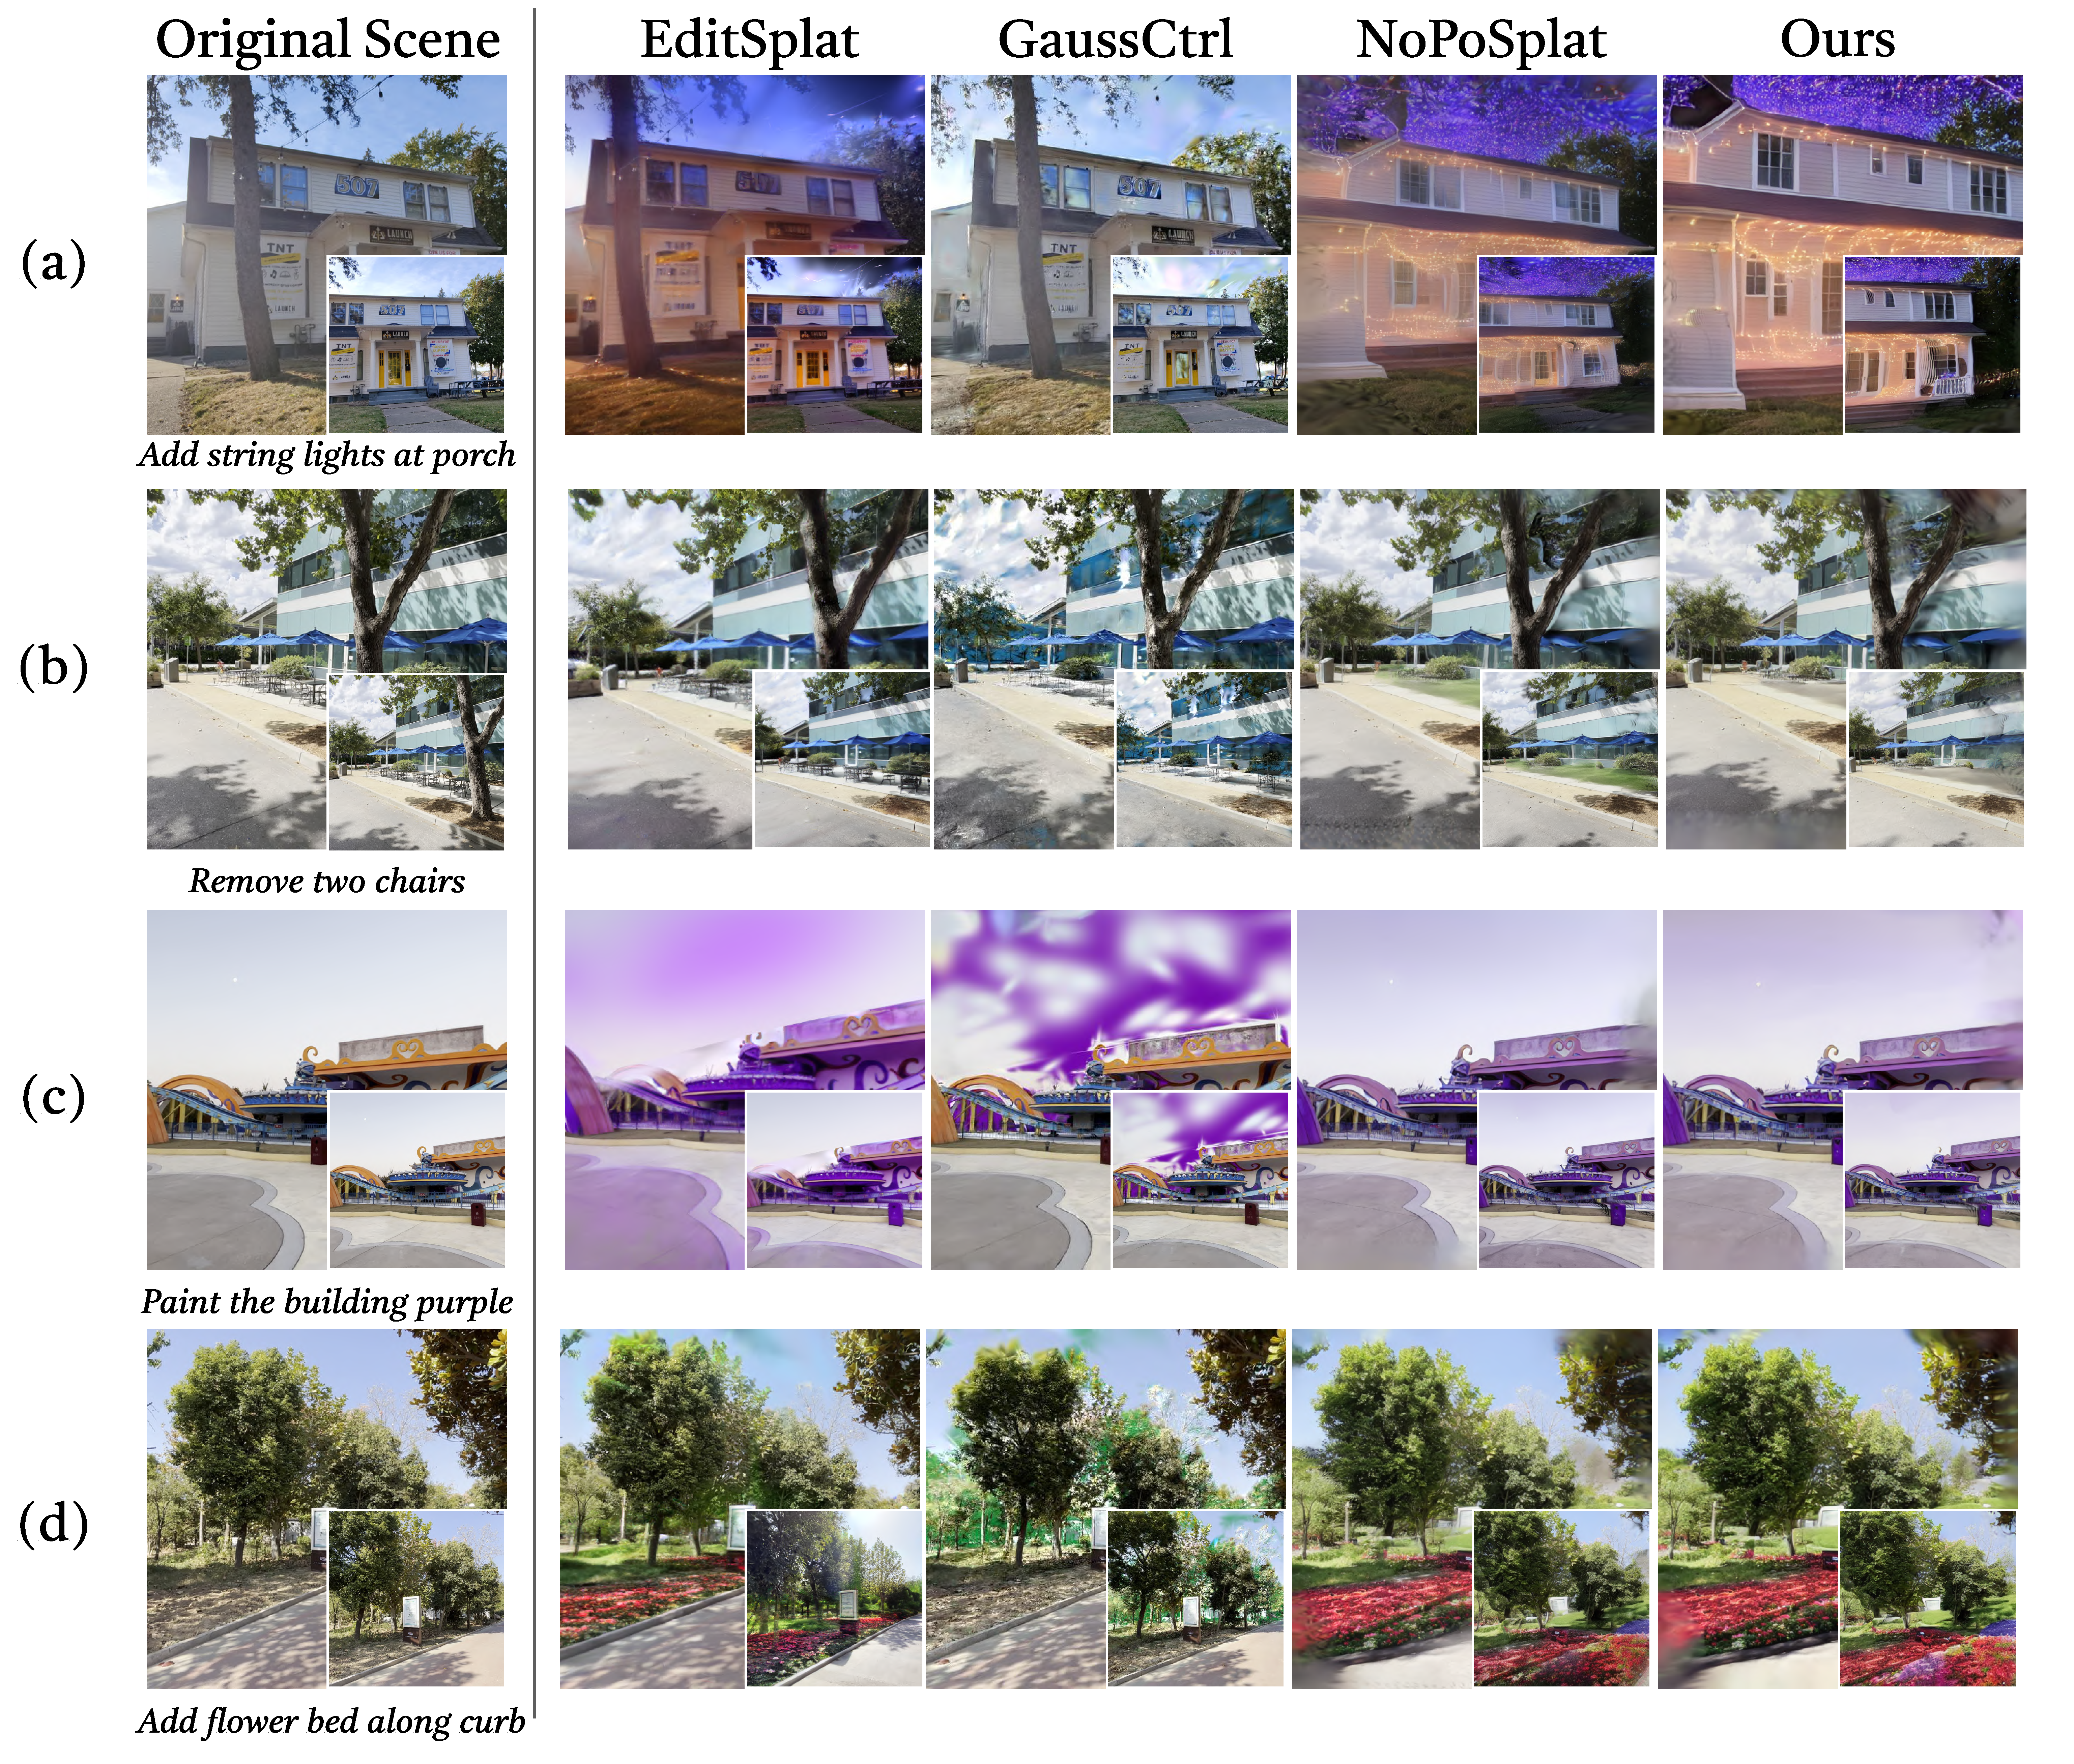
\includegraphics[width=0.93\textwidth]{fig/qualitative_comparison_v4.pdf}
    \caption{\textbf{Qualitative comparison} among four methods. The first row shows the original scene and the editing prompt; the remaining four rows show the results, each paired with an additional view.}
    \label{fig:qualitative-examples}
\end{figure*}

\subsection{Main Experiments} 
\vspace{1mm}
\noindent\textbf{Evaluation Metrics.} Similar to prior works~\cite{lee2025editsplatmultiviewfusionattentionguided, gaussctrl, in2n, you2025instainpaintinstant3dsceneinpainting}, we evaluate effectiveness from two angles: (1) whether the method performs the intended scene edits; (2) whether the 3D reconstruction is plausible across viewpoints. For (1), acknowledging the subjectivity of 3D scene generation, we adopt CLIP~\cite{radford2021learningtransferablevisualmodels} image-text similarity, which scores the absolute alignment between the edited render and the target description. For (2), we report C-FID~\cite{heusel2018ganstrainedtimescaleupdate}, which measures distribution-level realism by computing the Fréchet distance between feature distributions of edited renders and reference views, and C-KID~\cite{bińkowski2021demystifyingmmdgans}, which measures the kernel MMD between the same feature distributions and is more reliable with moderate sample sizes. Here, the prefix "C-" indicates that both metrics are computed in a scene-conditioned manner. Together they quantify overall realism/naturalness across views.

\vspace{1mm}
\noindent\textbf{Quantitative Comparison.} As summarized in Tab.~\ref{tab:main}, {\ourmethod} achieves the best quality-speed trade-off.
%
In terms of runtime, feed-forward methods are dramatically faster than optimization-based ones; 
{\ourmethod} processes a view in 0.51\,s (vs.\ 325.53\text{–}584.46\,s for optimization-based baselines). 
{\ourmethod} also attains the highest CLIP$_{t2i}$(text prompts to rendered images), indicating stronger instruction following and more effective scene edits. 
By design, GaussianCtrl applies only minor modifications, which keeps outputs close to the original and thus boosts C-FID and C-KID, but it underperforms on text alignment due to limited edit strength. 
EditSplat makes moderate edits and is relatively stable, yet remains conservative overall. 
NoPoSplat focuses on reconstruction rather than explicit editing; when input views are inconsistent, it tends to average conflicting evidence, producing blurred renders and uniformly lower scores (CLIP$_{t2i}$, C-FID and C-KID). 
Overall, {\ourmethod} best balances instruction following with multi-view realism, improving C-FID and C-KID over other feed-forward baselines while preserving semantics and structure nearly as well as the most conservative optimizer.

\vspace{1mm}
\noindent\textbf{Qualitative Comparison.}
Fig.~\ref{fig:qualitative-examples} presents four examples (a–d) of scene editing by EditSplat~\cite{lee2025editsplatmultiviewfusionattentionguided}, GaussCtrl~\cite{gaussctrl}, NoPoSplat~\cite{noposplat}, and {\ourmethod}. The small inset at the bottom-right of each panel shows the result from another viewpoint of the same scene. EditSplat achieves partially successful edits in (a, c, d), but it also alters regions that should remain unchanged, such as the sky and ground in (c). GaussCtrl is almost entirely unsuccessful across (a–d), producing chaotic or ineffective edits when applied to scenes that are unseen during its training. NoPoSplat generally generates plausible results, but its quality is highly sensitive to the inconsistency between input views: when cross-view inconsistency is large, it suffers from blur in (a,d), whereas for more consistent inputs in (b,c), the reconstruction quality is much better. In contrast, our method delivers stable, high-quality edits across all four scenes, maintaining consistency across views while preserving the original scene structure.

\begin{table}[t]
\centering
\scriptsize
\caption{\textbf{Quantitative comparison} on optimization-based and feed-forward methods.}
\label{tab:main}
\setlength{\tabcolsep}{6pt}
\renewcommand{\arraystretch}{1.1}
% \resizebox{\textwidth}{!}{%
\begin{tabular}{l@{\hskip 1.0mm}l@{\hskip 1.0mm}c@{\hskip 1.0mm}c@{\hskip 1.0mm}c@{\hskip 1.0mm}c}
\toprule
\textbf{Category} & \textbf{Method} &
\textbf{Time (s)}\,(\(\downarrow\)) &
\text{CLIP}$_{t2i}$(\(\uparrow\)) &
\textbf{C-FID}\,(\(\downarrow\)) &
\textbf{C-KID}\,(\(\downarrow\)) \\
\midrule
\multirow{2}{*}{Optimization}
& GaussCtrl~\cite{gaussctrl} & 325.53 & 0.227 & 135.0 & 0.091 \\
& Editsplat~\cite{lee2025editsplatmultiviewfusionattentionguided} & 584.46 & 0.241 & 174.1 & 0.122 \\
\midrule
\multirow{2}{*}{Feed-forward}
& NoPoSplat~\cite{noposplat} & 0.61   & 0.253 & 180.6 & 0.125 \\
& {\ourmethod} (Ours)   & 0.51   & 0.266 & 171.3 & 0.116 \\
\bottomrule
\vspace{-4mm}
\end{tabular}%
% }
\end{table}


\begin{table}[t]
\centering
\scriptsize
\caption{\textbf{Ablation quantitative comparison} on different training strategies in our method.}
\label{tab:training_ablation}
\setlength{\tabcolsep}{6pt}
\renewcommand{\arraystretch}{1.1}
\begin{tabular}{l@{\hskip 8.0mm}c@{\hskip 8.0mm}c@{\hskip 8.0mm}c}
\toprule
\textbf{Method} & \textbf{CLIP$_{t2i}$~(\(\uparrow\))} &
\textbf{C-FID~(\(\downarrow\))} & \textbf{C-KID~(\(\downarrow\))} \\
\midrule
{\ourmethod}  & 0.266 & 171.3 & 0.116 \\
+w/o Recolor   & 0.243 & 215.0 & 0.141 \\ %场景出现模糊
+w/o 3D Loss   & 0.237 & 278.4 & 0.182 \\ %场景歪的非常厉害
+w/o SAM  & 0.248 & 179.6 & 0.127 \\ %表现略微下降
+w/o R-Drop & 0.252 & 183.1 & 0.130 \\ %场景出现歪，深度出问题，view差距大了会出错，表现几乎不变
\bottomrule
\vspace{-4mm}
\end{tabular}
\end{table}

\subsection{Ablation Study}
We validate our design choices by comparing {\ourmethod} against different training and inference variants. Unless otherwise stated, the default configuration uses SAM2-based recoloring for supervision, the asymmetric input scheme, our full training losses (2D appearance + 3D regularization), randomly dropping the first view's Gaussian with $p{=}0.5$ during training; and InstructPix2Pix as the editing front-end at inference.

\vspace{1mm}
\noindent\textbf{Recolor/Image Editing For Training.}
Directly training on multi-view images produced by a 2D editor inevitably introduces substantial cross-view inconsistencies that act as label noise and hinder convergence. We therefore supervise training with \emph{SAM2-based recoloring}: object masks are extracted and recolored consistently across views, yielding stable, view-aligned targets. As Table \ref{tab:training_ablation} shows, in our ablations, replacing recoloring data with direct multi-view editing degrades multi-view consistency and increases artifacts, confirming the need for view-consistent supervision.

\vspace{1mm}
\noindent\textbf{Training Loss.} 
Because recoloring/editing can shift predicted Gaussian centers, relying solely on 2D losses (reconstruction/style) permits geometry drift: the rendering may look plausible while Gaussian primitives misalign in 3D. We ablate our 3D regularizers, and results are shown in Tab.~\ref{tab:training_ablation} . Removals lead to larger center deviation and diminished cross-view coherence. Using the full loss stabilizes geometry and improves semantic fidelity without sacrificing appearance.

\vspace{1mm}
\noindent\textbf{SAM2 Segmentation For Augmentation.}
To narrow the distribution gap between recolored training images and edited images at inference, we augment training data with SAM2-derived mask jittering (dilation/erosion), palette perturbation, and limited background leakage. Ablating these SAM2-based augmentations by training with plain recoloring only, reduces robustness and increases failure cases under stronger edits, indicating that modest variability during training is beneficial. Results are shown in Tab.~\ref{tab:training_ablation}.

\vspace{1mm}
\noindent\textbf{Random Drop the First View's Gaussian.}
Given the asymmetric inputs, the edited reference view can dominate the learned style. We introduce random drop during training: with probability $0.5$, we discard the Gaussians associated with the first view when forming supervision, forcing the network to propagate the edit semantics from the reference to the auxiliaries. Ablations on the drop probability, results in Tab.~\ref{tab:training_ablation}, show that removing random drop causes overfitting to the reference viewpoint, while excessively high drop rates weaken edit strength.

\begin{figure}[t]  % [t] 顶端
\scriptsize
    \centering
    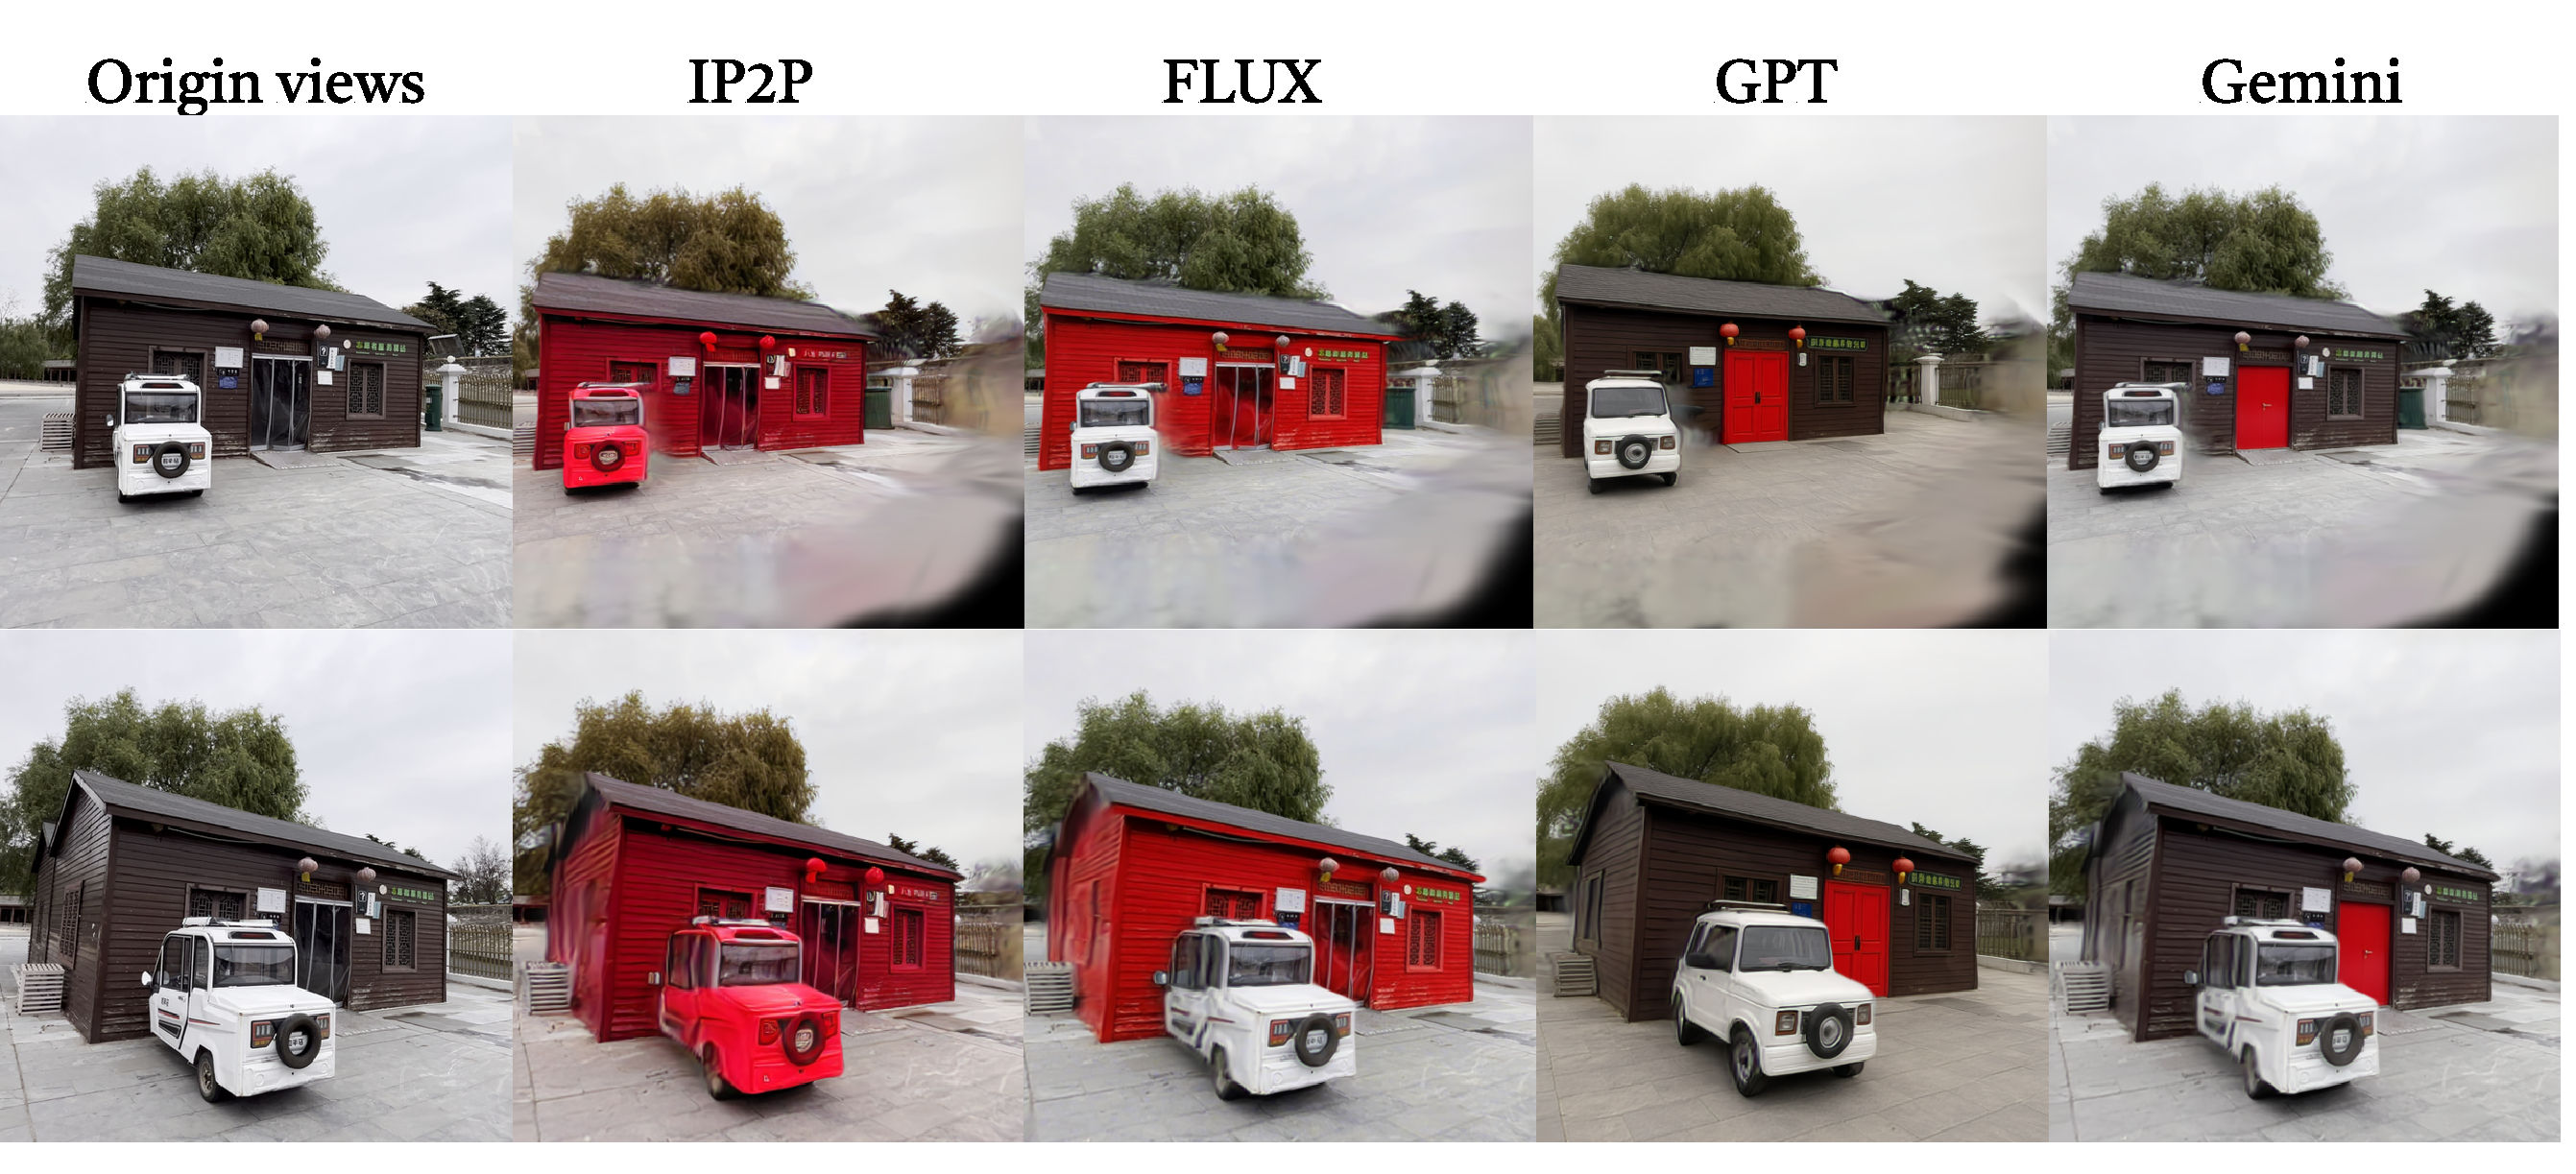
\includegraphics[width=\linewidth]{fig/image_editor.pdf}
    \caption{\textbf{Ablation qualitative comparison} among four image editors. \textit{Prompt: Paint the door red.}}
    \label{fig:image-editor}
    \vspace{-4mm}
\end{figure}

\vspace{1mm}
\noindent\textbf{Image Editing For Inference.}
Our pipeline decouples 2D editing from feed-forward reconstruction, allowing different editors at test time. We evaluate IP2P~\cite{ip2p} and alternatives including (1) OpenAI GPT-Image-1~\cite{gpt4o} (GPT) (2) Google Gemini-2.5-Flash-Image~\cite{geminiteam2025geminifamilyhighlycapable} (Gemini) (3) FLUX~\cite{labs2025flux1kontextflowmatching}. 
As shown in Fig.\ref{fig:image-editor} and Tab.\ref{tab:image_editor}, FLUX produces the highest visual edit quality but its edited regions are sometimes mislocalized; GPT and Gemini accurately identify the intended edit regions but tend to modify other parts of the image, while IP2P yields weak perceptual edit quality among the four.
Across editors, {\ourmethod} preserves its advantages in speed and consistency; stronger editors can improve local edit quality, while our model continues to enforce cross-view coherence. This indicates that {\ourmethod} is editor-agnostic and can benefit from future improvements in 2D editing.

\begin{table}[t]
\centering
\scriptsize
\caption{\textbf{Ablation quantitative comparison} on different image editors in our method.}
\vspace{-2mm}
\label{tab:image_editor}
\setlength{\tabcolsep}{6pt}
\renewcommand{\arraystretch}{1.1}

\begin{tabular}{l@{\hskip 8.0mm}c@{\hskip 8.0mm}c@{\hskip 8.0mm}c}
\toprule
\textbf{Method} & \textbf{CLIP$_{t2i}$~(\(\uparrow\))} &
\textbf{C-FID~(\(\downarrow\))} & \textbf{C-KID~(\(\downarrow\))} \\
\midrule
IP2P~\cite{ip2p}  & 0.266 & 171.3 & 0.116 \\
GPT~\cite{gpt4o}    & 0.261 & 166.2 & 0.102 \\ Gemini~\cite{geminiteam2025geminifamilyhighlycapable}  & 0.246 & 150.3 & 0.098 \\
FLUX~\cite{labs2025flux1kontextflowmatching}  & 0.276 & 169.9 & 0.112 \\
\bottomrule
\end{tabular}
\vspace{-4mm}
\end{table}
%